\documentclass[12pt,a4paper]{article}

\usepackage[utf8]{inputenc}
\usepackage[T1]{fontenc}
\usepackage{geometry}
\usepackage{graphicx}
\usepackage{booktabs}
\usepackage{array}
\usepackage{amsmath}
\usepackage{hyperref}
\usepackage{float}
\usepackage{caption}
\usepackage{subcaption}
\usepackage{parskip}
\usepackage{xcolor}
\usepackage{fancyhdr}
\usepackage{titlesec}
\usepackage{listings}

\geometry{top=2.5cm,bottom=2.5cm,left=2.5cm,right=2.5cm}

\pagestyle{fancy}
\fancyhf{}
\rhead{\small Introducción a la Ciencia de Datos}
\lhead{\small Grupo 10 --- Tarea 2}
\cfoot{\thepage}
\renewcommand{\headrulewidth}{0.4pt}

\titleformat{\section}{\large\bfseries}{}{0em}{}[\titlerule]
\titleformat{\subsection}{\normalsize\bfseries}{\thesubsection.}{0.5em}{}

\lstset{basicstyle=\small\ttfamily,backgroundcolor=\color{gray!10},frame=single,breaklines=true,columns=fullflexible,keepspaces=true}

\hypersetup{colorlinks=true,linkcolor=black,urlcolor=blue}

\begin{document}

\begin{titlepage}
  \centering
  \vspace*{2cm}
  {\large \textsc{Introducción a la Ciencia de Datos} \par}
  \vspace{1.5cm}
  {\Huge \bfseries INFORME TAREA 2: Clasificación de \\ artículos de prensa \par}
  \vspace{2cm}
  {\large Bruno Fabre Hernandez \\[0.3em] Santiago Burgueño Paysse \par}
  \vspace{2cm}
  {\large 25 de Junio 2026 \par}
  \vfill
\end{titlepage}

\tableofcontents
\newpage

\section*{Introducción}
\addcontentsline{toc}{section}{Introducción}

Esta tarea es la continuación de la Tarea 1. Se utilizan los mismos datos del dataset \textit{All the News 2.1} y la función \texttt{clean\_text()} desarrollada previamente. El objetivo es aplicar técnicas de representación numérica de texto y entrenar modelos de clasificación para predecir a qué medio de prensa pertenece cada artículo.

\section{Parte 1: Dataset y representación numérica de texto}

\subsection{Preparación del dataset}

Se trabajó con los tres medios de prensa con mayor cantidad de artículos del dataset:

\begin{table}[H]
  \centering
  \begin{tabular}{lr}
    \toprule
    \textbf{Medio} & \textbf{Artículos totales} \\
    \midrule
    Reuters & 9.431 \\
    The New York Times & 2.840 \\
    CNBC & 2.623 \\
    \bottomrule
  \end{tabular}
  \caption{Medios seleccionados y cantidad de artículos.}
\end{table}

Se aplicó la función \texttt{clean\_text()} de la Tarea 1 sobre la combinación de título y cuerpo del artículo. Esta función elimina el dateline, convierte a minúsculas, elimina URLs y puntuación, y colapsa espacios múltiples.

El dataset resultante (14.894 artículos) se particionó en \textbf{70\% train} y \textbf{30\% test} con muestreo estratificado (\texttt{stratify=y, random\_state=42}), garantizando que la proporción de cada medio se mantenga igual en ambos conjuntos:

\begin{table}[H]
  \centering
  \begin{tabular}{lr}
    \toprule
    \textbf{Partición} & \textbf{Artículos} \\
    \midrule
    Train & 10.425 \\
    Test  & 4.469 \\
    \bottomrule
  \end{tabular}
  \caption{Tamaño de las particiones train y test.}
\end{table}

\subsection{Verificación del balance de clases}

\begin{figure}[H]
  \centering
  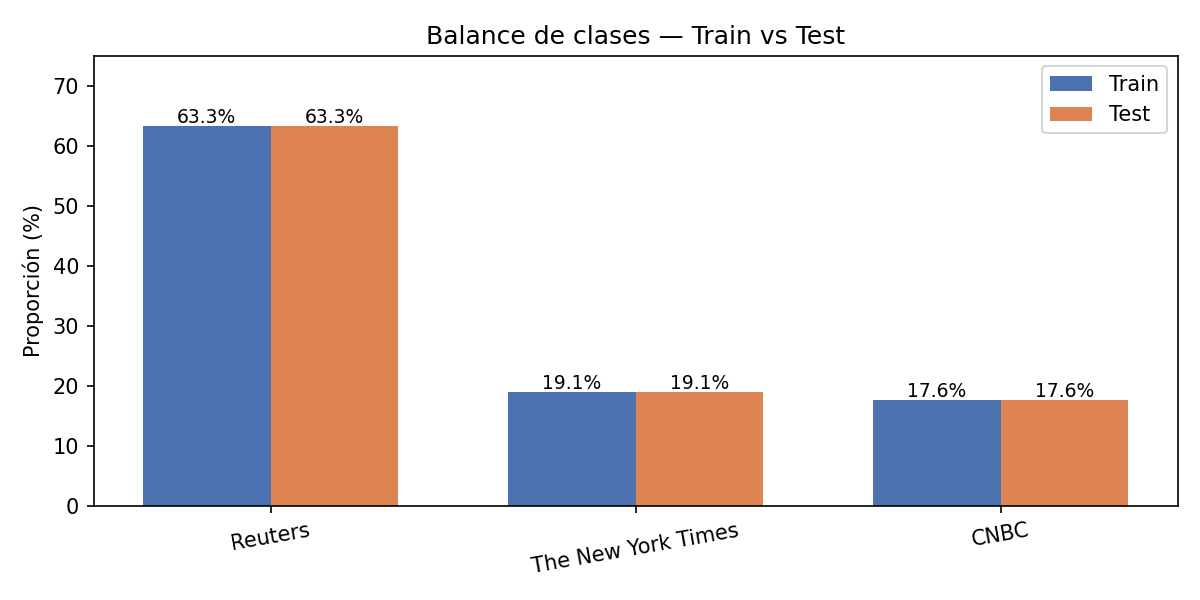
\includegraphics[width=0.92\textwidth]{imgs/fig1_balance.png}
  \caption{Balance de clases en los conjuntos de train y test.}
\end{figure}

El gráfico confirma que la estratificación funcionó correctamente: las proporciones de cada medio son prácticamente idénticas en train y test. Reuters representa aproximadamente el 63\% del dataset, mientras que NYT y CNBC representan alrededor del 19\% y 18\% respectivamente. Este desbalance tendrá implicancias importantes en el comportamiento de los modelos, como se analizará en la Parte 2.

\subsection{Representación Bag of Words}

Bag of Words (BoW) representa cada artículo como un vector de conteos sobre el vocabulario construido a partir del conjunto de entrenamiento, produciendo una \textbf{matriz documento-término} de dimensión artículos $\times$ términos. La representación es inherentemente \textit{sparse} --- cada artículo activa solo una fracción pequeña del vocabulario total --- y descarta el orden de las palabras: el modelo captura presencia y frecuencia, pero no estructura sintáctica ni contexto.

El vectorizador se ajusta (\texttt{fit}) únicamente sobre el conjunto de entrenamiento y se aplica (\texttt{transform}) sobre el test, evitando filtración de información entre ambas particiones.

\begin{table}[H]
  \centering
  \begin{tabular}{lr}
    \toprule
    \textbf{Dimensión} & \textbf{Valor} \\
    \midrule
    Artículos (filas) & 10.425 \\
    Palabras en vocabulario (columnas) & 86.698 \\
    Celdas totales & $\sim$904 millones \\
    Celdas no-nulas & 0,247\% \\
    \bottomrule
  \end{tabular}
  \caption{Dimensiones de la matriz BoW del conjunto de entrenamiento.}
\end{table}

Almacenar la matriz completa en formato denso requeriría varios GB de RAM. Una representación \textit{sparse} guarda únicamente los valores no-nulos junto con sus coordenadas, reduciendo el uso de memoria en más de 400 veces.

\subsection{Representación TF-IDF}

Un \textbf{n-grama} es una secuencia de $N$ palabras consecutivas. Con \texttt{ngram\_range=(1,2)} el vectorizador considera tanto palabras individuales (unigramas) como pares de palabras adyacentes (bigramas). Por ejemplo, ``nueva york'' como bigrama captura información que se perdería tratando ``nueva'' y ``york'' como términos independientes.

TF-IDF mejora BoW penalizando palabras muy frecuentes en todos los documentos y premiando palabras específicas de ciertos artículos. El \textbf{TF} (\textit{Term Frequency}) mide la frecuencia de la palabra en el documento actual; el \textbf{IDF} (\textit{Inverse Document Frequency}) penaliza palabras que aparecen en muchos documentos --- palabras como ``the'' o ``said'' tienen IDF cercano a 0. El peso final $\text{TF-IDF} = \text{TF} \times \text{IDF}$ resulta alto para palabras frecuentes en un artículo pero raras en el corpus.

Se utilizó la configuración \texttt{stop\_words=``english''}, \texttt{use\_idf=True}, que adicionalmente elimina las palabras más comunes del inglés antes de la vectorización. El vocabulario TF-IDF resultante tiene \textbf{86.393 términos}.

\subsection{Visualización SVD sobre TF-IDF}

Tras aplicar TF-IDF, cada artículo queda representado como un vector de 86.393 dimensiones --- un espacio imposible de visualizar directamente. Para explorar si los artículos de los tres medios forman grupos distinguibles, se aplicó \textbf{Singular Value Decomposition} (SVD), una técnica de álgebra lineal que reduce la dimensionalidad del espacio preservando la mayor cantidad posible de su estructura.

SVD opera proyectando todos los artículos sobre las direcciones del espacio donde los datos presentan mayor dispersión entre sí. La primera componente (SVD1) captura la dirección de máxima varianza; la segunda (SVD2) captura la segunda dirección más informativa, con la restricción de ser perpendicular a SVD1 para no redundar en la misma información. Al retener solo 2 componentes, cada artículo queda representado por un par de coordenadas que puede graficarse.

Estas coordenadas son combinaciones lineales de miles de términos y no tienen una interpretación semántica directa. Lo que sí es interpretable es la posición relativa entre artículos: puntos cercanos en el gráfico comparten un perfil de vocabulario similar.

Se utilizó \textbf{TruncatedSVD} en lugar de PCA clásico porque opera directamente sobre matrices \textit{sparse}, evitando la conversión a formato denso que PCA requiere y que produciría un error de memoria con matrices de estas dimensiones.

\subsubsection*{Comparación de configuraciones}

\begin{figure}[H]
  \centering
  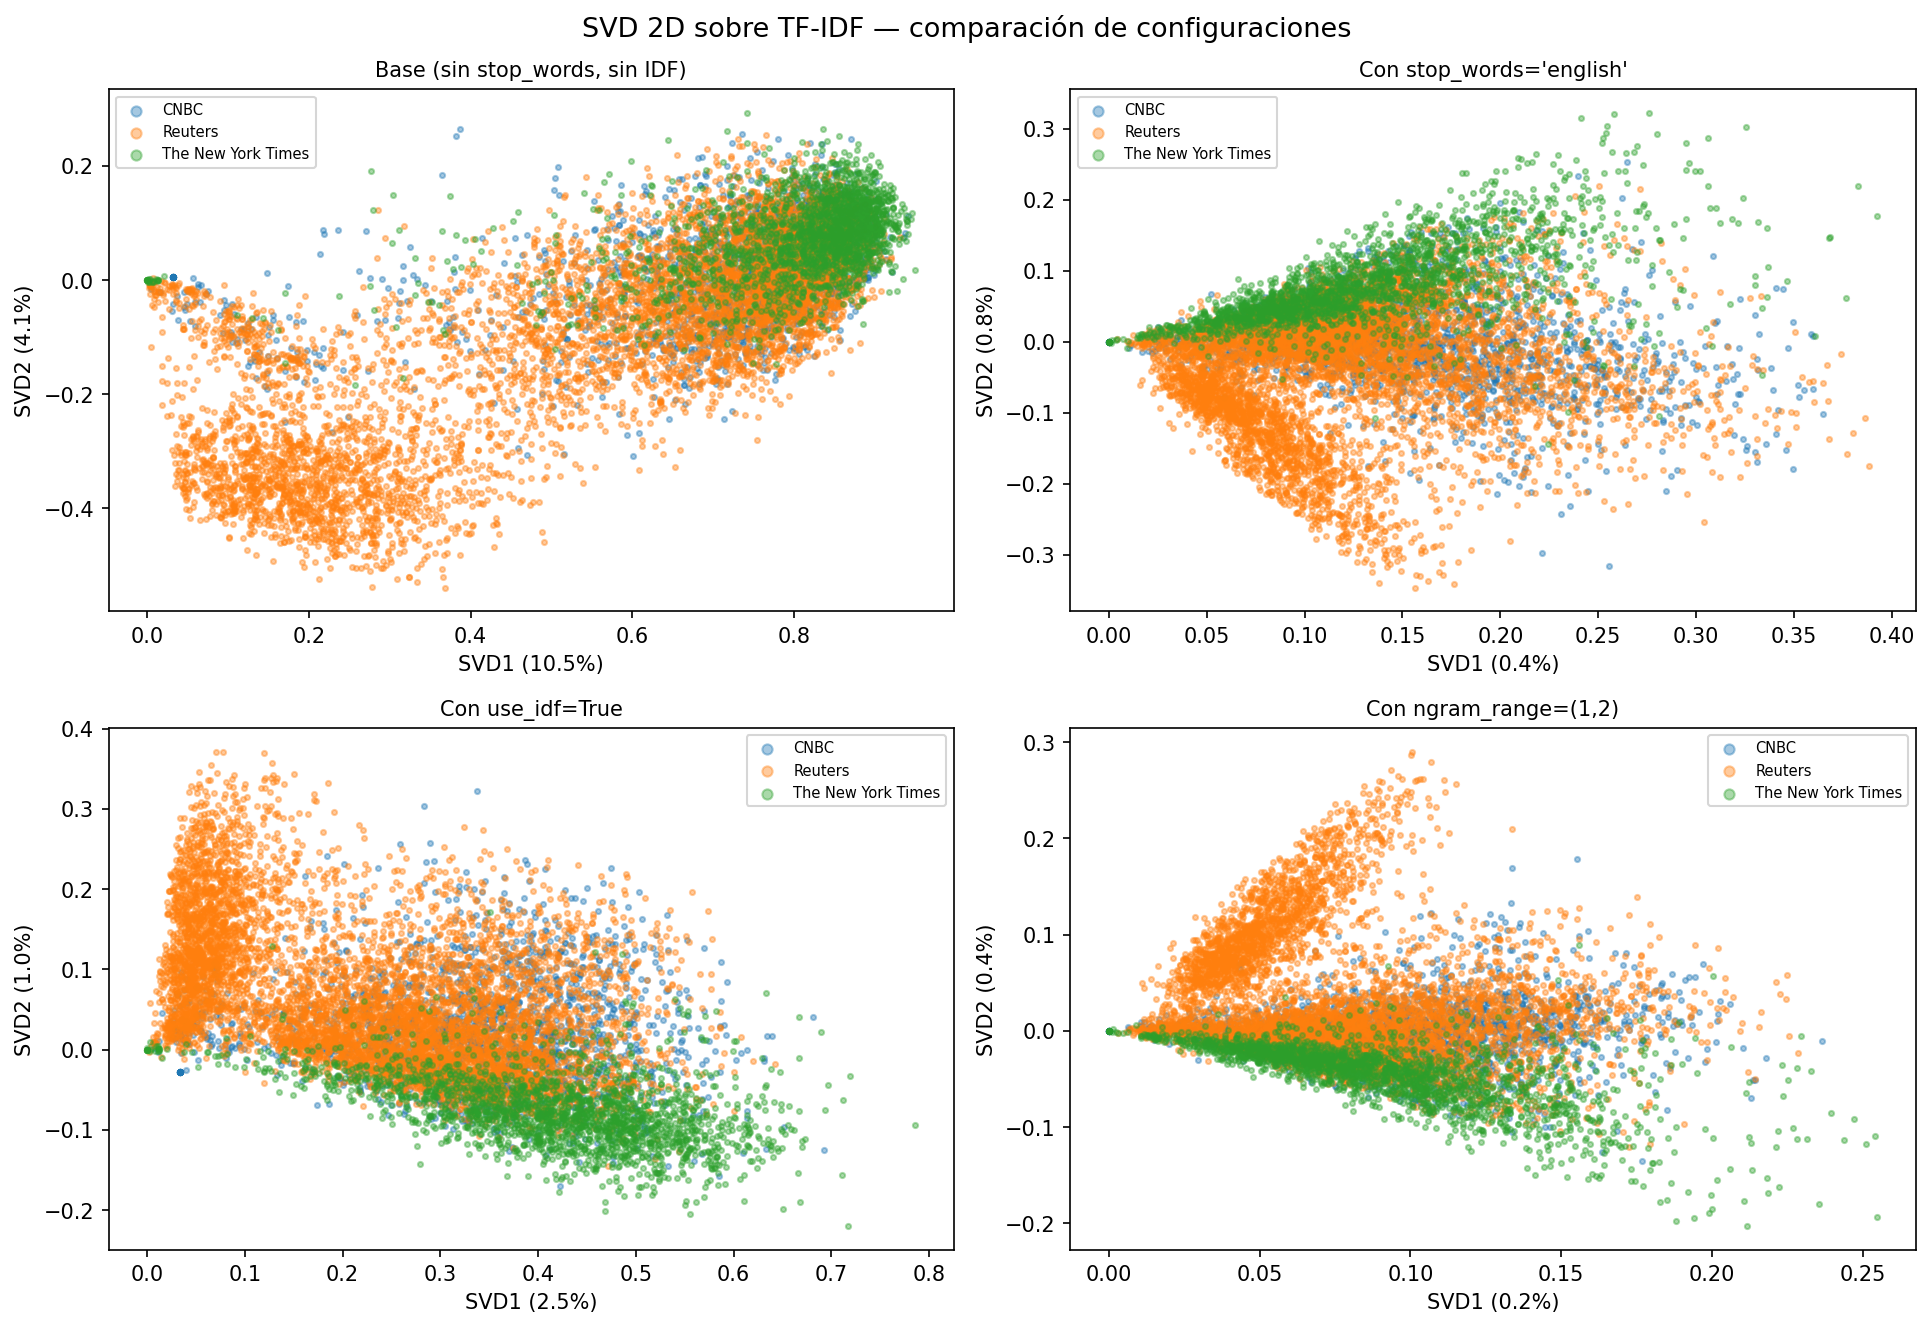
\includegraphics[width=\textwidth]{imgs/fig2_svd_configs.png}
  \caption{Visualización SVD (2 componentes) con cuatro configuraciones de vectorización TF-IDF.}
\end{figure}

En todos los gráficos se observa superposición considerable entre los tres medios. Esto no implica que el problema de clasificación sea difícil, sino que \textbf{2 componentes son insuficientes} para capturar la separación real que existe en las 86.393 dimensiones originales.

Sin \textit{stop words} ni IDF, SVD1 captura el 10,5\% de la varianza, dominada por palabras muy frecuentes. Al agregar \textit{stop words}, esa varianza se redistribuye hacia términos más informativos y SVD1 cae a 0,4\%. Con bigramas el vocabulario se expande y la varianza se distribuye aún más --- SVD1 explica solo el 0,2\%.

\subsubsection*{Varianza explicada}

\begin{figure}[H]
  \centering
  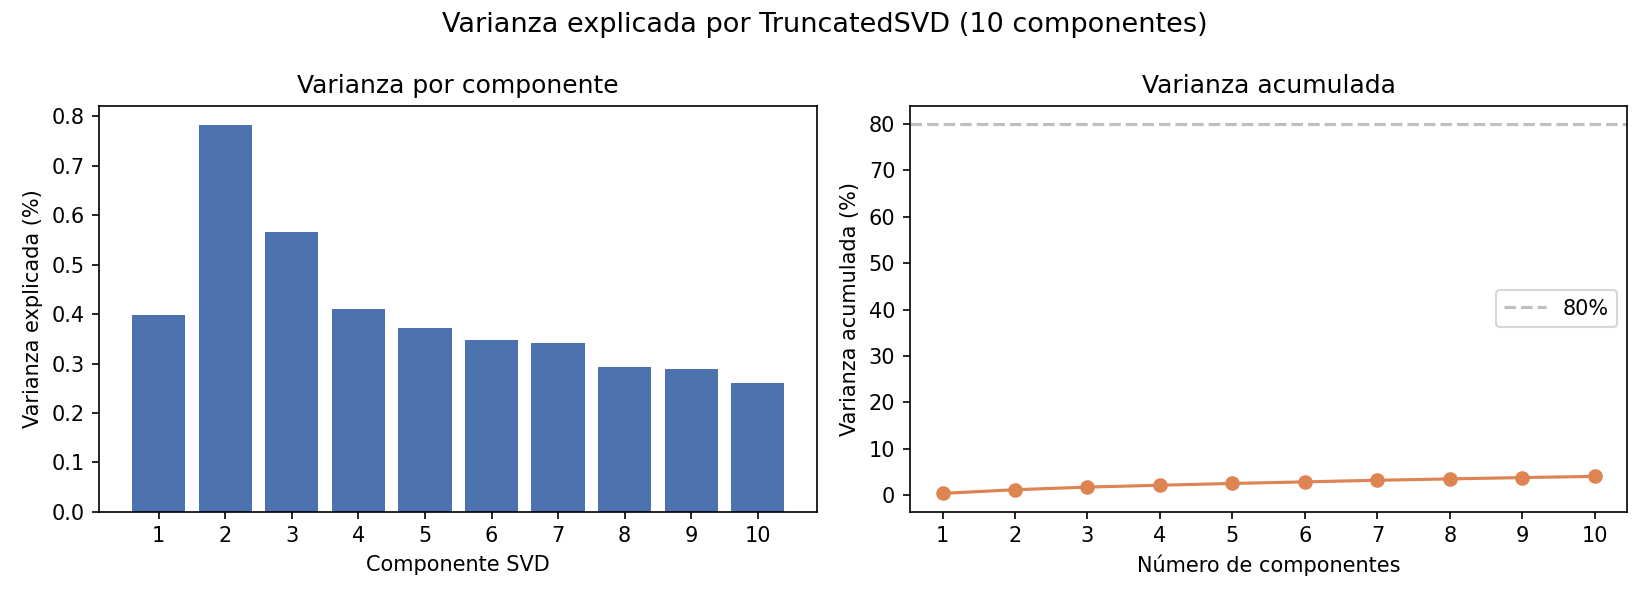
\includegraphics[width=0.92\textwidth]{imgs/fig3_varianza.png}
  \caption{Varianza explicada acumulada por TruncatedSVD con hasta 10 componentes.}
\end{figure}

Con 10 componentes, TruncatedSVD explica apenas el \textbf{4,06\% de la varianza total}. Esto indica que la información discriminativa no está concentrada en pocas dimensiones sino distribuida de forma muy homogénea. La superposición visual entre clases en los gráficos 2D no refleja la dificultad real del problema: los modelos de la Parte 2 logran separar los medios con un rendimiento significativamente mejor del que los gráficos sugerirían.

\section{Parte 2: Entrenamiento y Evaluación de Modelos}

\subsection{Multinomial Naive Bayes}

Naive Bayes aplica el teorema de Bayes: dado un artículo con ciertas palabras, calcula la probabilidad de que pertenezca a cada clase y elige la de mayor probabilidad. Se llama ``naive'' porque asume independencia condicional entre palabras --- cada término contribuye de forma independiente a la probabilidad de la clase.

El parámetro \texttt{alpha} controla el suavizado de Laplace: evita que palabras no vistas en el entrenamiento colapsen la probabilidad de una clase a cero.

\medskip
\noindent\textbf{Resultados con \texttt{alpha=1.0} (valor por defecto):}

\begin{table}[H]
  \centering
  \begin{tabular}{lcccc}
    \toprule
    \textbf{Medio} & \textbf{Precision} & \textbf{Recall} & \textbf{F1} & \textbf{Support} \\
    \midrule
    CNBC              & 1,00 & 0,02 & 0,04 & 787  \\
    Reuters           & 0,70 & 1,00 & 0,82 & 2830 \\
    The New York Times & 0,95 & 0,45 & 0,61 & 852  \\
    \midrule
    \textbf{Accuracy} & \multicolumn{3}{c}{\textbf{0,7203}} & \textbf{4469} \\
    \bottomrule
  \end{tabular}
  \caption{Métricas por clase --- Naive Bayes con \texttt{alpha=1.0}.}
\end{table}

\begin{figure}[H]
  \centering
  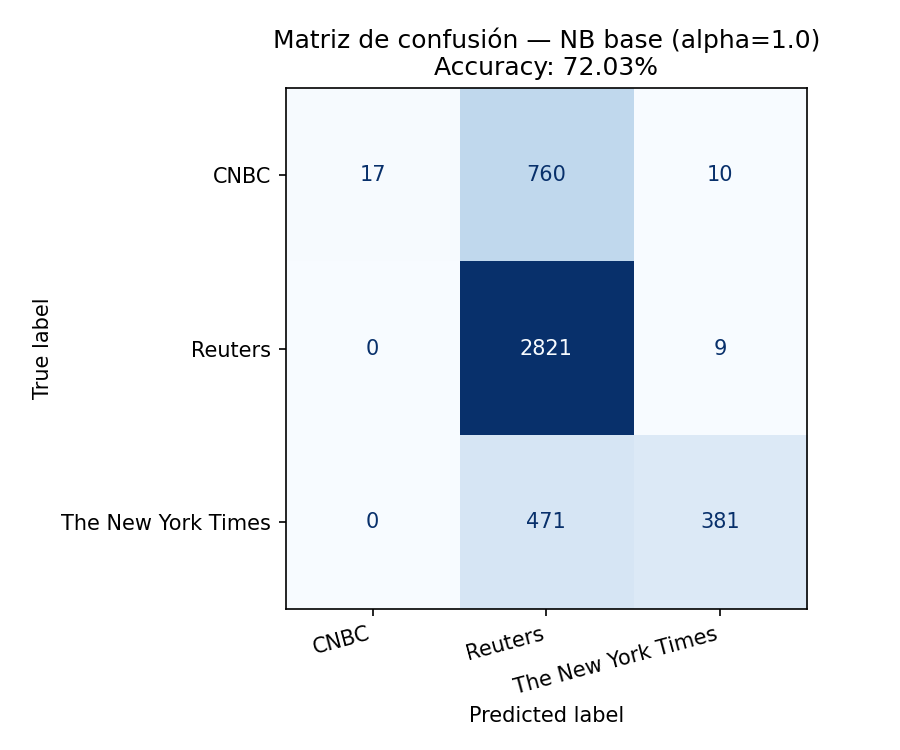
\includegraphics[width=0.65\textwidth]{imgs/fig4_cm_nb_base.png}
  \caption{Matriz de confusión --- Naive Bayes con \texttt{alpha=1.0}.}
\end{figure}

Los resultados revelan un modelo fuertemente sesgado hacia la clase mayoritaria. Reuters alcanza recall$=1{,}00$ pero precision$=0{,}70$: el modelo clasifica como Reuters gran parte de los artículos ante cualquier ambigüedad. En el extremo opuesto, CNBC es prácticamente ignorada --- recall$=0{,}02$ y F1$=0{,}04$ --- con el 98\% de sus artículos absorbidos por Reuters. NYT queda en una posición intermedia con recall$=0{,}45$.

El accuracy global del 72\% resulta engañoso dado el desbalance de clases: un clasificador trivial que prediga siempre Reuters alcanzaría el 63\% sin aprender ninguna estructura. El F1 macro de 0,49 refleja con más fidelidad la capacidad real del modelo.

\subsection{Validación cruzada y búsqueda de hiperparámetros}

Los resultados del modelo base muestran que el valor por defecto de \texttt{alpha} no es necesariamente el óptimo. Para encontrar el mejor hiperparámetro es necesario evaluar distintos valores --- pero esa evaluación no puede hacerse sobre el test, ya que el conjunto de test debe permanecer completamente aislado hasta el final. En su lugar, la selección de hiperparámetros se realiza sobre el \textbf{conjunto de validación}, construido mediante \textbf{cross-validation de 5 folds} dentro del train:

\begin{center}
\begin{lstlisting}
Dataset completo
+-- TRAIN (70%) <- cross-validation trabaja aca para elegir alpha
+-- TEST  (30%) <- intacto, solo se usa al final una vez
\end{lstlisting}
\end{center}

\textbf{GridSearchCV} automatiza este proceso para cada valor de \texttt{alpha}, entrenando en total $7 \times 5 = \mathbf{35}$ modelos:

\begin{table}[H]
  \centering
  \begin{tabular}{ccc}
    \toprule
    \textbf{Alpha} & \textbf{Accuracy promedio (CV)} & \textbf{Desv. estándar} \\
    \midrule
    0,01          & 0,8046 & 0,0042 \\
    \textbf{0,1}  & \textbf{0,8110} & \textbf{0,0035} \\
    0,5           & 0,7464 & 0,0061 \\
    1,0           & 0,7122 & 0,0044 \\
    2,0           & 0,6700 & 0,0025 \\
    5,0           & 0,6359 & 0,0009 \\
    10,0          & 0,6332 & 0,0002 \\
    \bottomrule
  \end{tabular}
  \caption{Resultados de GridSearchCV por valor de \texttt{alpha}. Mejor configuración en negrita.}
\end{table}

\begin{figure}[H]
  \centering
  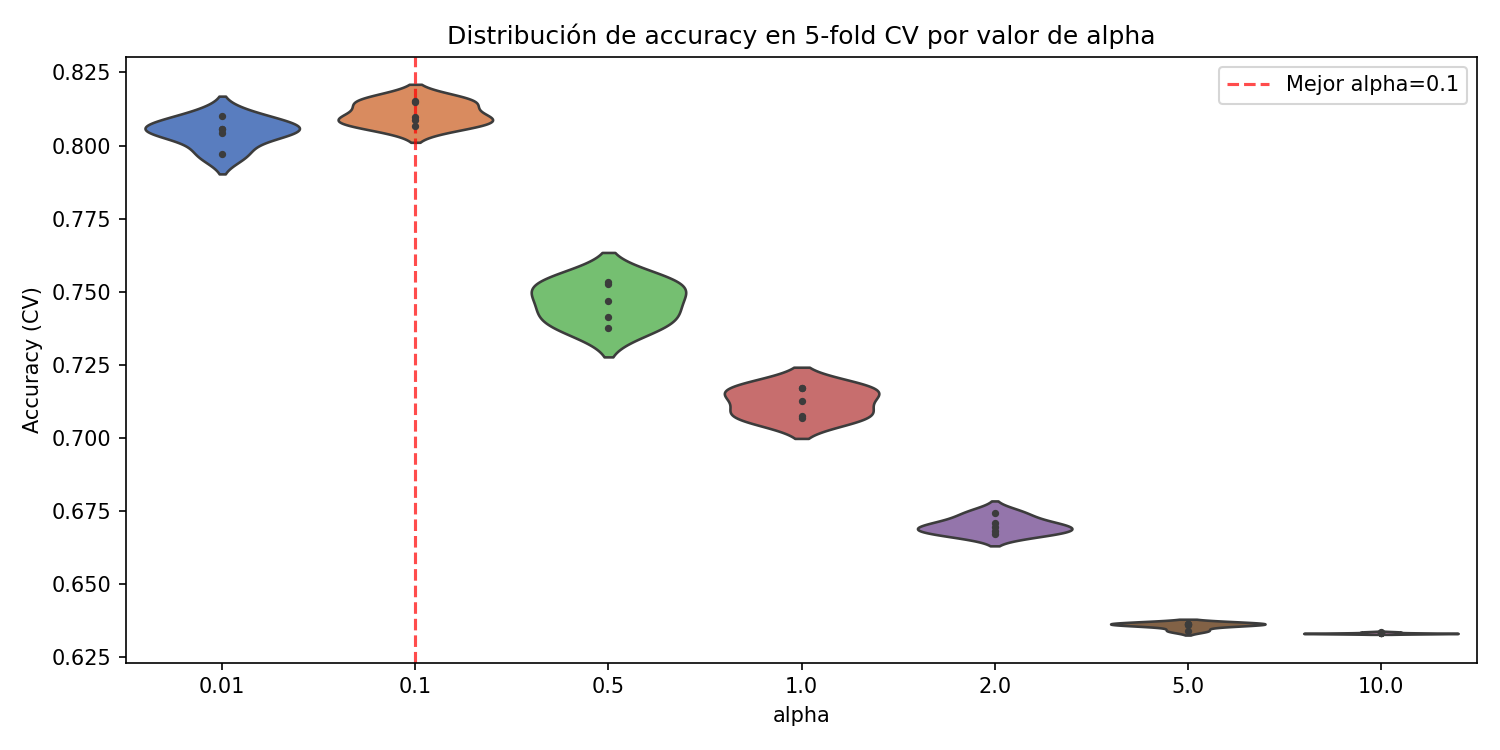
\includegraphics[width=0.88\textwidth]{imgs/fig5_violin.png}
  \caption{Distribución del accuracy en los 5 folds para cada valor de \texttt{alpha} (violin plot).}
\end{figure}

Alpha$=0{,}1$ tiene el mejor promedio con variabilidad razonable. Valores altos de \texttt{alpha} producen modelos demasiado simples que no capturan bien las diferencias entre clases.

\subsection{Entrenamiento final con el mejor modelo}

Con \texttt{alpha=0.1}, se reentrenó el modelo sobre \textbf{todo el conjunto de entrenamiento} y se evaluó por primera vez sobre el test:

\begin{table}[H]
  \centering
  \begin{tabular}{lcccc}
    \toprule
    \textbf{Medio} & \textbf{Precision} & \textbf{Recall} & \textbf{F1} & \textbf{Support} \\
    \midrule
    CNBC              & 0,84 & 0,33 & 0,47 & 787  \\
    Reuters           & 0,82 & 0,94 & 0,88 & 2830 \\
    The New York Times & 0,76 & 0,81 & 0,78 & 852  \\
    \midrule
    \textbf{Accuracy} & \multicolumn{3}{c}{\textbf{0,8085}} & \textbf{4469} \\
    \bottomrule
  \end{tabular}
  \caption{Métricas por clase --- Naive Bayes con \texttt{alpha=0.1} (modelo final).}
\end{table}

La mejora es significativa: de 72,03\% a \textbf{80,85\%} de accuracy, y el F1 macro pasó de 0,49 a 0,71. El recall de CNBC mejoró de 0,02 a 0,33.

\subsection{Modelo alternativo: Regresión Logística}

La Regresión Logística aprende un peso por cada término del vocabulario. Para clasificar un artículo, calcula un score como suma ponderada de sus valores TF-IDF y aplica la función \textit{softmax} para convertirlo en probabilidades. A diferencia de Naive Bayes, no asume independencia entre \textit{features} --- puede capturar correlaciones entre palabras.

\begin{table}[H]
  \centering
  \begin{tabular}{lcccc}
    \toprule
    \textbf{Medio} & \textbf{Precision} & \textbf{Recall} & \textbf{F1} & \textbf{Support} \\
    \midrule
    CNBC              & 0,88 & 0,51 & 0,65 & 787  \\
    Reuters           & 0,85 & 0,98 & 0,91 & 2830 \\
    The New York Times & 0,94 & 0,83 & 0,88 & 852  \\
    \midrule
    \textbf{Accuracy} & \multicolumn{3}{c}{\textbf{0,8711}} & \textbf{4469} \\
    \bottomrule
  \end{tabular}
  \caption{Métricas por clase --- Regresión Logística (\texttt{C=1.0, max\_iter=1000}).}
\end{table}

\begin{figure}[H]
  \centering
  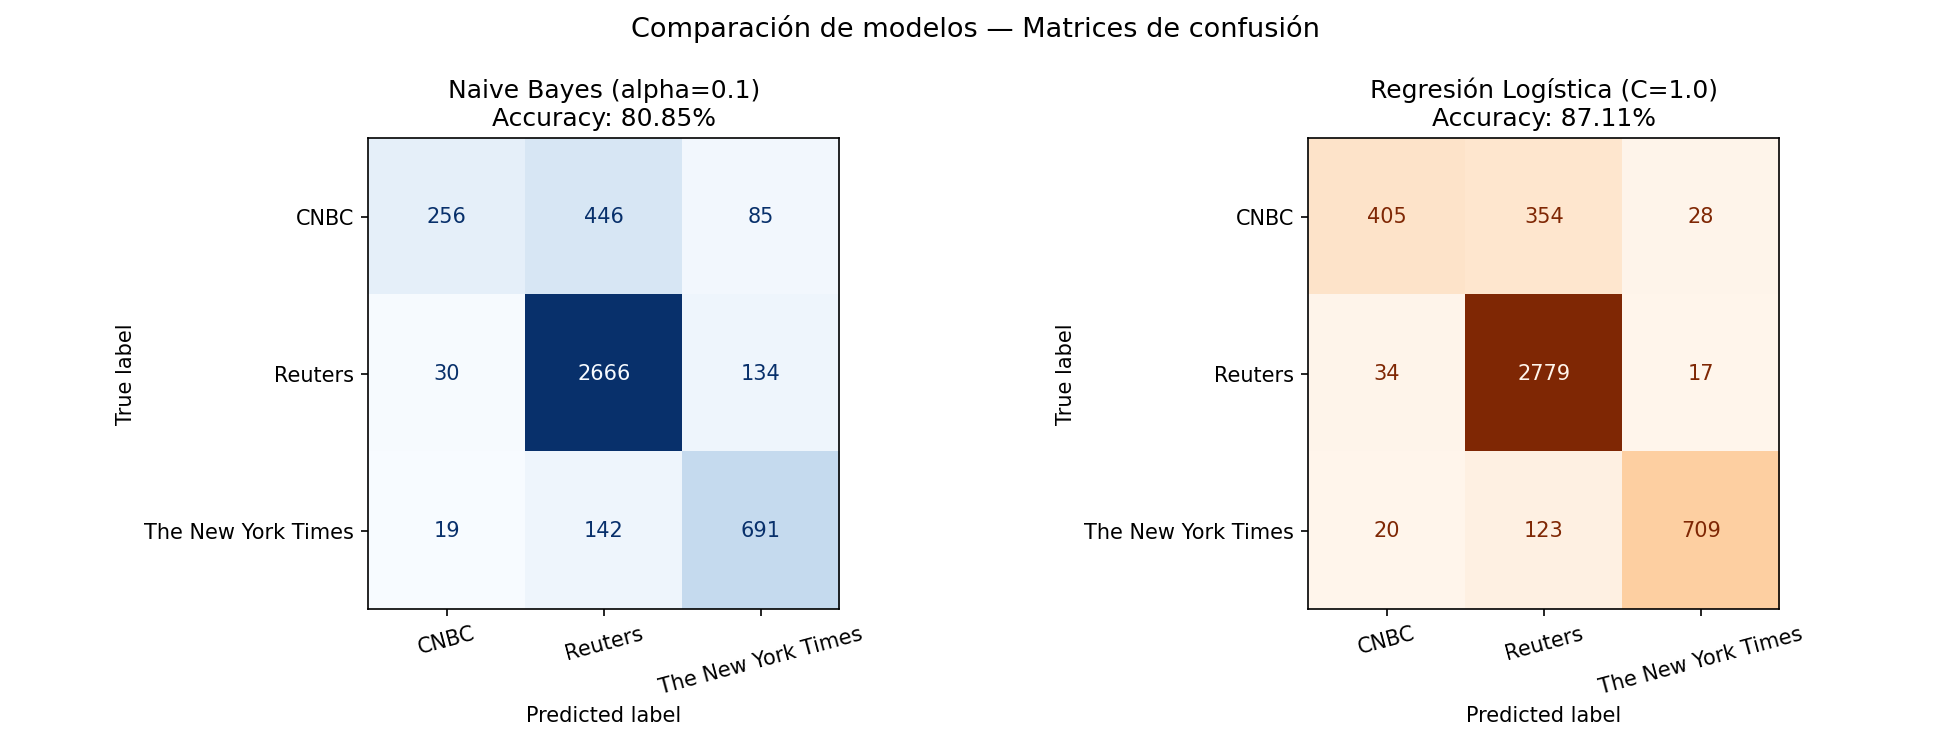
\includegraphics[width=\textwidth]{imgs/fig6_comparacion_modelos.png}
  \caption{Comparación de matrices de confusión: Naive Bayes (izq.) vs.\ Regresión Logística (der.).}
\end{figure}

La Regresión Logística supera al mejor Naive Bayes en todas las métricas: accuracy 87,11\% vs.\ 80,85\%, F1 macro 0,82 vs.\ 0,71. La mejora es especialmente notable en CNBC (recall 0,51 vs.\ 0,33).

\subsection{Cambio de medio de prensa}

Se evaluó el problema con \textbf{Reuters, People y Business Insider}, elegidos para introducir un desbalance más pronunciado:

\begin{table}[H]
  \centering
  \begin{tabular}{lr}
    \toprule
    \textbf{Medio} & \textbf{Artículos} \\
    \midrule
    Reuters          & 9.431 \\
    People           & 1.528 \\
    Business Insider & 660   \\
    \bottomrule
  \end{tabular}
  \caption{Medios alternativos y cantidad de artículos.}
\end{table}

\begin{figure}[H]
  \centering
  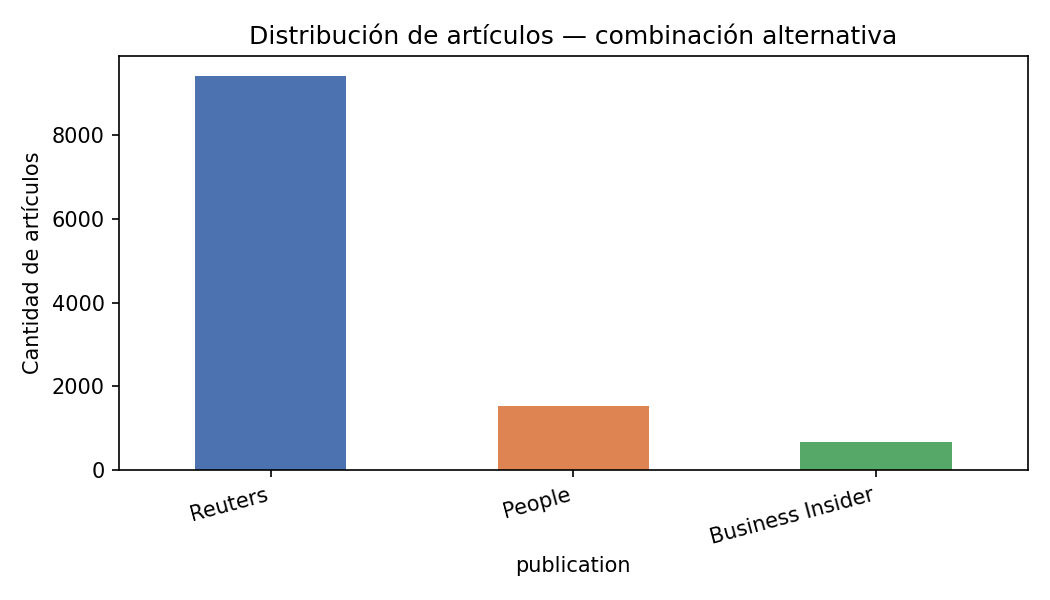
\includegraphics[width=0.78\textwidth]{imgs/fig7_balance_alt.png}
  \caption{Balance de clases --- combinación de medios alternativos.}
\end{figure}

\begin{table}[H]
  \centering
  \begin{tabular}{lcccc}
    \toprule
    \textbf{Medio} & \textbf{Precision} & \textbf{Recall} & \textbf{F1} & \textbf{Support} \\
    \midrule
    Business Insider & 0,97 & 0,31 & 0,47 & 198  \\
    People           & 0,85 & 0,93 & 0,89 & 458  \\
    Reuters          & 0,96 & 0,99 & 0,97 & 2830 \\
    \midrule
    \textbf{Accuracy} & \multicolumn{3}{c}{\textbf{0,9406}} & \textbf{3486} \\
    \bottomrule
  \end{tabular}
  \caption{Métricas por clase --- medios alternativos, Naive Bayes \texttt{alpha=0.1}.}
\end{table}

\begin{figure}[H]
  \centering
  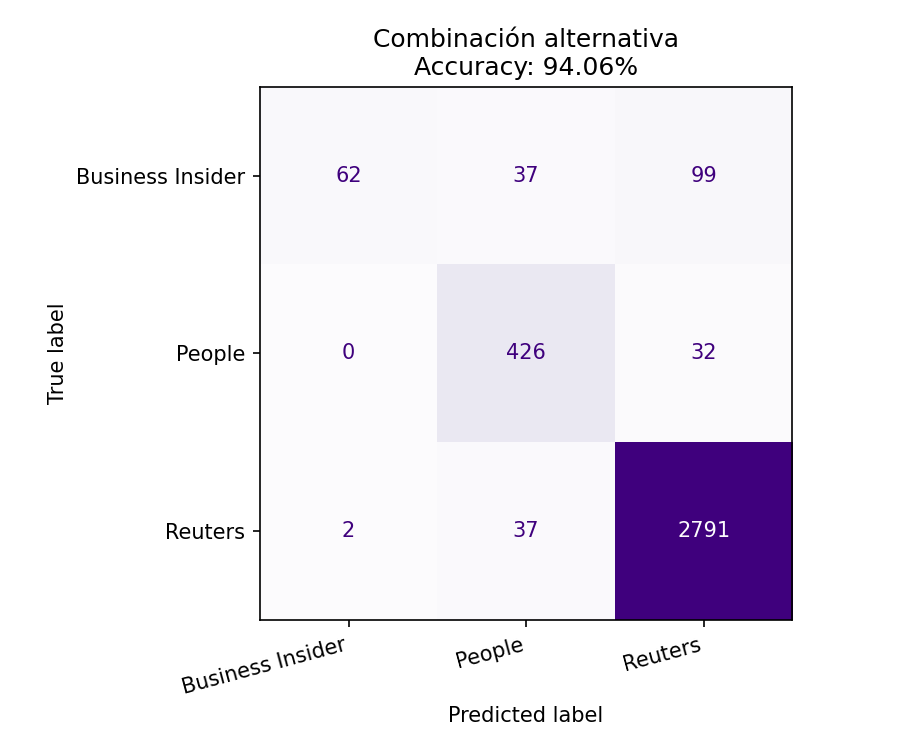
\includegraphics[width=0.65\textwidth]{imgs/fig8_cm_alt.png}
  \caption{Matriz de confusión --- medios alternativos.}
\end{figure}

El accuracy del 94\% es nuevamente engañoso dado que Reuters domina el dataset (81\% del test). Business Insider tiene recall de 0,31. People muestra resultados sorprendentemente buenos (recall$=0{,}93$), probablemente porque su vocabulario de entretenimiento es muy distinto al de Reuters.

Para mitigar el desbalance existen técnicas como \textit{oversampling} (SMOTE), \textit{undersampling}, o usar \texttt{class\_weight=`balanced'} en scikit-learn.

\subsection{Técnica alternativa de extracción de features: Word Embeddings}

Los \textbf{word embeddings} (Word2Vec, GloVe, FastText, BERT) representan cada palabra como un vector denso de baja dimensión (típicamente 100--300 dimensiones), aprendido de grandes corpus de texto. A diferencia de TF-IDF, los embeddings capturan similitud semántica: palabras con significados parecidos tienen vectores cercanos en el espacio. Modelos más avanzados como BERT además producen un vector distinto para la misma palabra según el contexto en que aparezca.

\subsection{Clasificación a nivel de título}

Se repitió el pipeline completo utilizando únicamente el \textbf{título del artículo}:

\begin{table}[H]
  \centering
  \begin{tabular}{lc}
    \toprule
    \textbf{Configuración} & \textbf{Accuracy} \\
    \midrule
    Artículo completo (NB, \texttt{alpha=0.1}) & 80,85\% \\
    Solo título (NB, \texttt{alpha=0.1})        & 72,59\% \\
    \bottomrule
  \end{tabular}
  \caption{Comparación de accuracy: artículo completo vs.\ solo título.}
\end{table}

\begin{figure}[H]
  \centering
  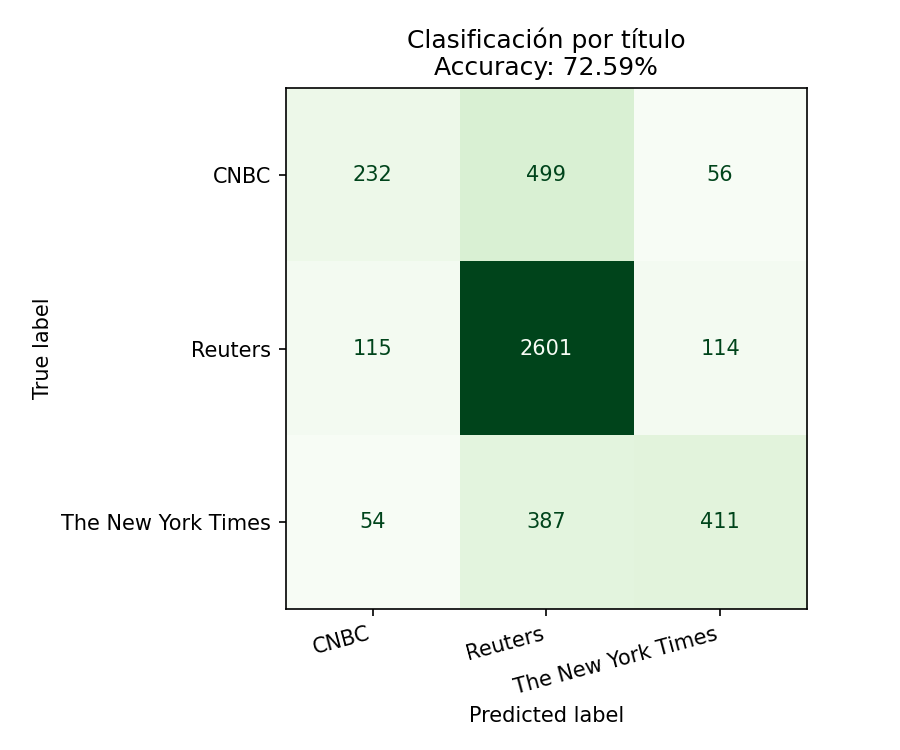
\includegraphics[width=0.65\textwidth]{imgs/fig9_cm_titulo.png}
  \caption{Matriz de confusión --- clasificación usando solo el título del artículo.}
\end{figure}

La caída de $\sim$8 puntos de accuracy es esperable dado que el título contiene mucha menos información. Aun así, un 72,6\% de accuracy clasificando solo por título indica que los medios tienen estilos de titular diferenciados.

\section*{Conclusiones}
\addcontentsline{toc}{section}{Conclusiones}

La representación TF-IDF con eliminación de \textit{stop words} es una base sólida para clasificación de texto, alcanzando un 80,85\% de accuracy con Naive Bayes optimizado. La Regresión Logística supera claramente a Naive Bayes (87,11\% vs.\ 80,85\%), sugiriendo que las correlaciones entre términos son informativas para esta tarea.

El desbalance de clases es el principal desafío del problema: Reuters domina el dataset y los modelos tienden a clasificar hacia esa clase. El accuracy solo no es una métrica suficiente --- el F1 por clase revela información que el accuracy oculta.

Con solo 2 componentes SVD se explica menos del 2\% de la varianza del espacio TF-IDF, lo que confirma que la separabilidad entre medios existe pero requiere muchas más dimensiones de las que se pueden visualizar.

\end{document}
